\chapter{Nmpc-codegen}
This chapter describes the software library that was written for this thesis. First an overview of the workflow and the functionality of the library is given. Followed by a in-depth description of the implementation.
\section{Overview library}
The nmpc-codegen library contains a framework to construct a Python script that generates a MPC controller. This controller uses the panoc algorithm to solve the optimization problem.

Figure~\ref{fig:nmpc-codegen scheme} illustrates how this is accomplished. On the left side is the Python or Matlab script that the user will construct. It contains the mathematical model nd the control parameters of the process that needs to be controlled.The output of the Python script is displayed on the right side in figure~\ref{nmpc-codegen scheme}. The output contains some static code, which is mostly associated with the panoc algorithm. And some dynamic code which is generated in Python and will differ from problem to problem. Finally sometimes the output will also contain simulation tools, this optional feature allows the user to simulate the controller from within Python or Matlab.
	\begin{figure}[H]
		\centering
		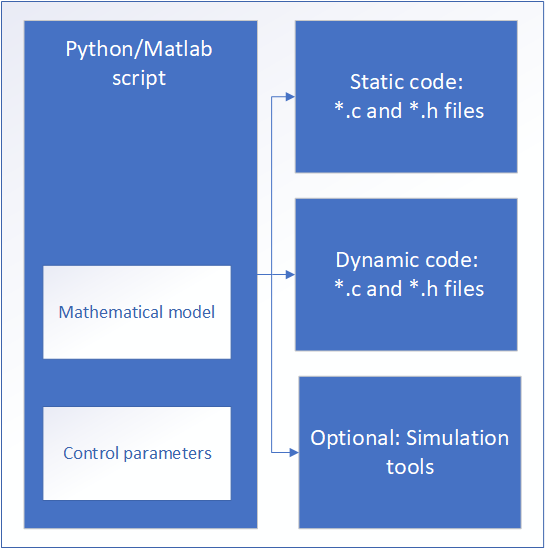
\includegraphics[width=0.5\textwidth]{nmpc_codegen_scheme}
		\caption{nmpc-codegen scheme}
		\label{fig:nmpc-codegen scheme}
	\end{figure}

\section{Casadi}
The panoc algorithm is a derivative driven algorithm, this means that the gradient of the cost function must be available to the algorithm. This gradient is generated using backward automatic differentiation.

\subsection{Algorithmic differentiation (AD)}
There exists a number of ways to determine the derivative of a function. The most obvious way is using symbolic differentiation. This method has been used over more than 200 years to calculate the gradient by hand. But in order to use symbolic differentiation, the algorithm needs one mathematical defined function. Which might be hard to get.

Another way of calculating derivatives, is through numerical differentiation also known as the method of finite differences. Although this method is very simple to implement, the accuracy is not always sufficient. And the method is rather slow if there are lots of partial derivatives.

An second alternative way to calculate the derivatives is through automatic differentiation. This method has two variants forward automatic differentiation and backward automatic differentiation.

The simplest of the two is forward differentiation, the only requirement to use this algorithm is that the entire function must be expressed in elementary operations. This is something computers are naturally good at. Equation~\ref{eq:example used with automatic differentiation} illustrates a simple example of such function. Two intermediate valuables are used to express the elementary operations.
\begin{equation}
	\begin{aligned}
		& y = a \cdot b + cos(b) \\
		& x_1 = a \cdot b \\
		& x_2 = cos(b) \\
		& y = x_1 + x_2		
	\end{aligned}
	\label{eq:example used with automatic differentiation}
\end{equation}
Forward automatic differentiation gets its name from the fact that the chain rule is applied from input to output. It derives from the lowest variables to the highest viable. As illustrated by equation~\ref{eq:math definition forward automatic differentation}. Equation~\ref{eq:example forward automatic differentiation} contains a worked out example of this algorithm. The first line of equation~\ref{eq:example forward automatic differentiation} contains the theoretical answer. The  following two lines contain the derivatives of the intermediate variables towards the b variable. Finally the to the derivatives are summed up and deserved it towards b is found.

The problem with forward automatic differentiation is that for each variable all the intermediate derivatives needs to be calculated. This is where the idea for backward automatic differentiation came from. As it allows to generate the derivative to all inputs variables in one big sweep. Although it's more expensive to calculate one single derivative, it is cheaper to calculate all the derivatives.

\begin{equation}
	\frac{dx_i}{db} = \frac{dx_i}{dx_j}\frac{dx_j}{dx_k}\frac{dx_k}{db}
	\label{eq:math definition forward automatic differentation}
\end{equation}

\begin{equation}
	\begin{aligned}
		& \frac{\partial y}{\partial b} = a - sin(b) \\
		& \frac{\partial x_1}{\partial b} = a  \\
		& \frac{\partial x_2}{\partial b} = -sin(b) \\
		& \frac{\partial y}{\partial b} = \frac{\partial x_1}{\partial b} + \frac{\partial x_2}{\partial b}	 = a - sin(b)
	\end{aligned}
	\label{eq:example forward automatic differentiation}
\end{equation}

Backward automatic differentiation is the opposite of forward automatic differentiation as it works down from the output towards the input. As illustrated by equation~\ref{eq:math definition backward automatic differentation}. An example is worked out in equation~\ref{eq:example backward automatic differentiation}. Even if there are hundreds of intermediate variables it only required one line to find a component of the gradient. This is the main reason why packages like casadi use backward automatic differential, instead of forward.

\begin{equation}
	\frac{\partial x_i}{\partial b} = \frac{\partial x_i}{\partial x_k}\frac{\partial x_k}{\partial x_j}\frac{\partial x_j}{\partial b}
	\label{eq:math definition backward automatic differentation}
\end{equation}

\begin{equation}
\begin{aligned}
& \bar{x_1} = \bar{x_3} \frac{\partial x_3}{\partial x_1} = 1 \cdot 1 \\
& \bar{x_2} = \bar{x_3} \frac{\partial x_3}{\partial x_2} = 1 \cdot 1 \\
& \frac{\partial y}{\partial b} = \bar{x_1} \frac{\partial x_1}{\partial b} + \bar{x_2} \frac{\partial x_2}{\partial b} = a - sin(b)\\
& \frac{\partial y}{\partial a} = \bar{x_1} \frac{\partial x_1}{\partial a} = b
\end{aligned}
\label{eq:example backward automatic differentiation}
\end{equation}

The same example can be calculated with Casadi as demonstrated in listing~\ref{lst:casadi demo backward automatic differentiation} with output in table~\ref{tbl:output casadi demo backward automatic differentiation}. The intermediate variables are @1,@2 and @3. output[0][0] is the function value and input[1][0] and input[1][1] is the gradient. 

\begin{lstlisting}[caption={Casadi example automatic backward differentiation},label={lst:casadi demo backward automatic differentiation}]
a = cd.SX.sym('a',(1,1))
b = cd.SX.sym('b',(1,1))
y = a*b + cd.cos(b)
f = cd.Function('f',[a,b],[y,cd.gradient(y,cd.vertcat(a,b))])
print(f)
\end{lstlisting}


\begin{table}
	\begin{center}
		\begin{tabular}{ |l|  }
			\hline
			Output Casadi code listing~\ref{lst:casadi demo backward automatic differentiation} \\
			\hline
			Number of inputs: 2 \\
			Input 0 ("i0"): 1-by-1 (dense) \\
			Input 1 ("i1"): 1-by-1 (dense) \\
			Number of outputs: 2 \\
			Output 0 ("o0"): 1-by-1 (dense) \\
			Output 1 ("o1"): 2-by-1 (dense) \\
			@0 = input[0][0]; \\
			@1 = input[1][0]; \\
			@2 = (@0*@1); \\
			@3 = cos(@1); \\
			@2 = (@2+@3); \\
			output[0][0] = @2; \\
			output[1][0] = @1; \\
			@1 = sin(@1); \\
			@0 = (@0-@1); \\
			output[1][1] = @0; \\
			\hline   
		\end{tabular}
		\label{tbl:output casadi demo backward automatic differentiation}
	\end{center}
\end{table}



\section{Nmpc-codegen implementation}
Nmpc-codegen exists out of a high-level language such as Python or Matlab that generates header files and source files. The higher-level language can call the build system (Cmake/make) to compile the generate code. In order to simulate the generated controller. At the end of the development cycle the Python/Matlab code can generate the controller without a build system. So that the code can easily be integrated into an existing project.

\subsection{Python and Matlab}
Figure~\ref{fig:nmpc_codegen_packages} Illustrates the architecture of the nmpc-codegen library. There are five sub packages tools, models, example models, controller and Cfunctions.  The two classes in the sub package models, represent the mathematical model of the system. The user must construct an object of one of these classes, that contains the function equation of the system.

The Cfunctions sub package contains proximal functions that represent constraints on the inputs. The user manual contains a table of all available constraints to the user. The tools sub package contains two classes. The bootstrapper can generate the static code, and the simulator that allows the user to call the generated C code from Python or Matlab.

The controller sub package contains the Nmpc\_panoc class, an object of this class represents the actual controller. In order to construct an object of the Nmpc\_panoc class the user must provide a model object, a proximal function object and one or two stage costs object.

Finally the user can also add obstacles, these will be added a soft constraints into the cost function. The obstacles can be found in the sub package obstacles from the sub package controller.
	\begin{figure}[H]
		\centering
		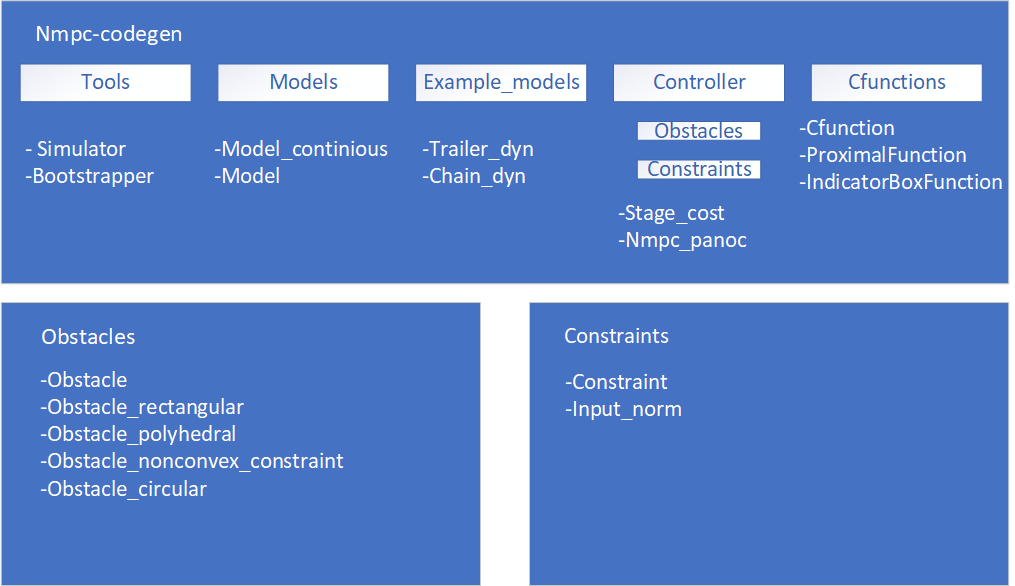
\includegraphics[width=1\textwidth]{nmpc_codegen_packages}
		\caption{Software architecture}
		\label{fig:nmpc_codegen_packages}
	\end{figure}

\subsection{C}
The C code is written in a layered architecture, the lowest layer contains the buffer, the cost function and the lipschitz estimator. The second layer contains the proximal gradient descent algorithm and the L-BFGS algorithm. The highest layer contains only the panoc algorithm.

Each of these entities has its own source file. The NMPC entity initializes the cost function with the current state of each iteration, and calls panoc. The end-user does not need to know how panoc or any of the underlying layers work. The NMPC entity takes care of everything, the user will simply call NMPC with the current state, a reference state, a reference input and output array to place the optimal inputs.
	\begin{figure}[H]
		\centering
		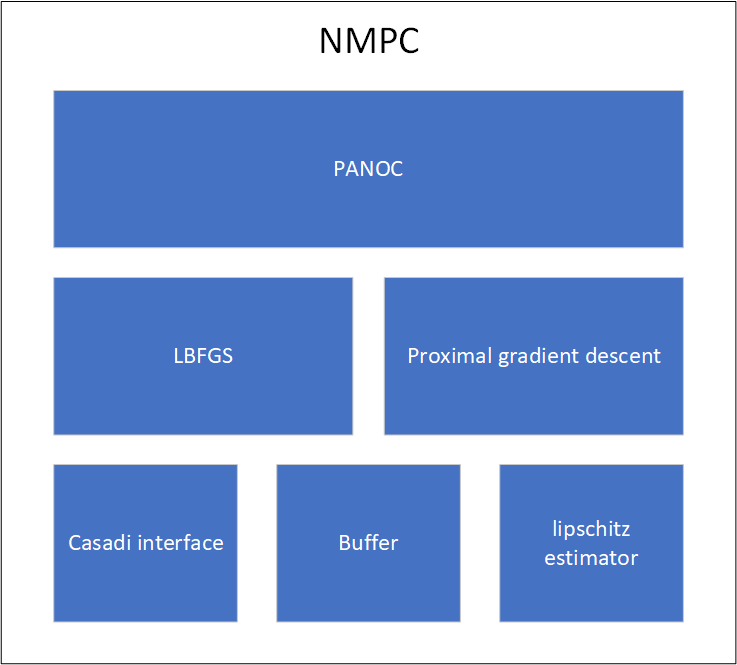
\includegraphics[width=0.5\textwidth]{visio_software_arch}
		\caption{Software architecture}
		\label{fig:visio software arch}
	\end{figure}
\subsection{Build system}
The build system must be compatible with Windows, Linux and Mac X os. This is why there was opted to use Cmake. As it can generate build systems for all three operating systems, using the available compilers. The structure of the build system is illustrated in figure~\ref{fig:build system}. Python or Matlab first calls Cmake to generate the Make files. After the make files are generated the Python or Matlab code calls the makefile to compile the controller code into a shared library.
\begin{figure}[H]
	\centering
	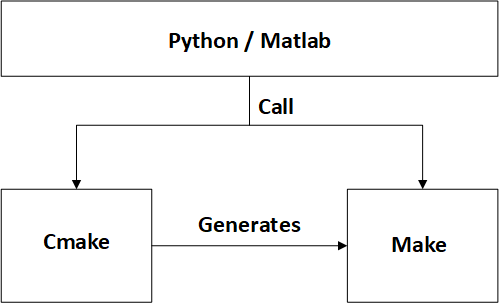
\includegraphics[width=0.5\textwidth]{build_system}
	\caption{Build system}
	\label{fig:build system}
\end{figure}
In order to easily simulate the controller from Python, the Python code must be able to call into a compile library. This is accomplished using the Ctypes library, which allows Python script to directly call C functions.(If the dynamic library has the necessary properties)

Matlab can also call directly into a dynamic library, this is accomplished through the callib function in Matlab. The same compiled shared library can be used for either Matlab or Python.

